% !TEX encoding = UTF-8
% !TEX TS-program = pdflatex
% !TEX root = ../Tesi.tex
% !TEX spellcheck = en-EN

%************************************************
\chapter{Blast Furnace}
\label{cap:blastfurnace}
%************************************************

\section{Blast furnace design}
\label{sec:bfdesign}

Well explained in the vast literature (\cite{RefWorks:203}), 
iron making consists in separating the iron from its chemical combination with
oxygen. 
As of now, the blast furnace (Fig. \ref{fig:125blastfurnace}) is considered the
most efficient process.

\begin{figure}[htbp]
\centering 
  \subfloat[Blast furnace scheme \cite{RefWorks:200}.]
  {
	  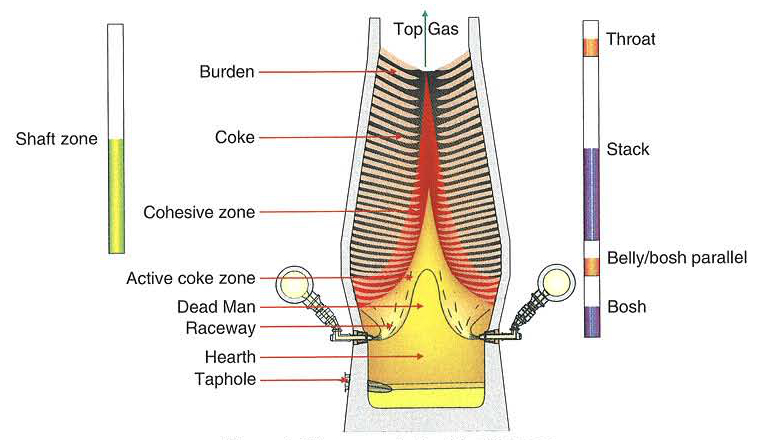
\includegraphics[width=.54\columnwidth]{images/125blastfurnace}
	  \label{fig:125blastfurnace}  }
  \quad
    \subfloat[Blast furnace section layout (Voestalpine Stahl GmbH).]
    {
	  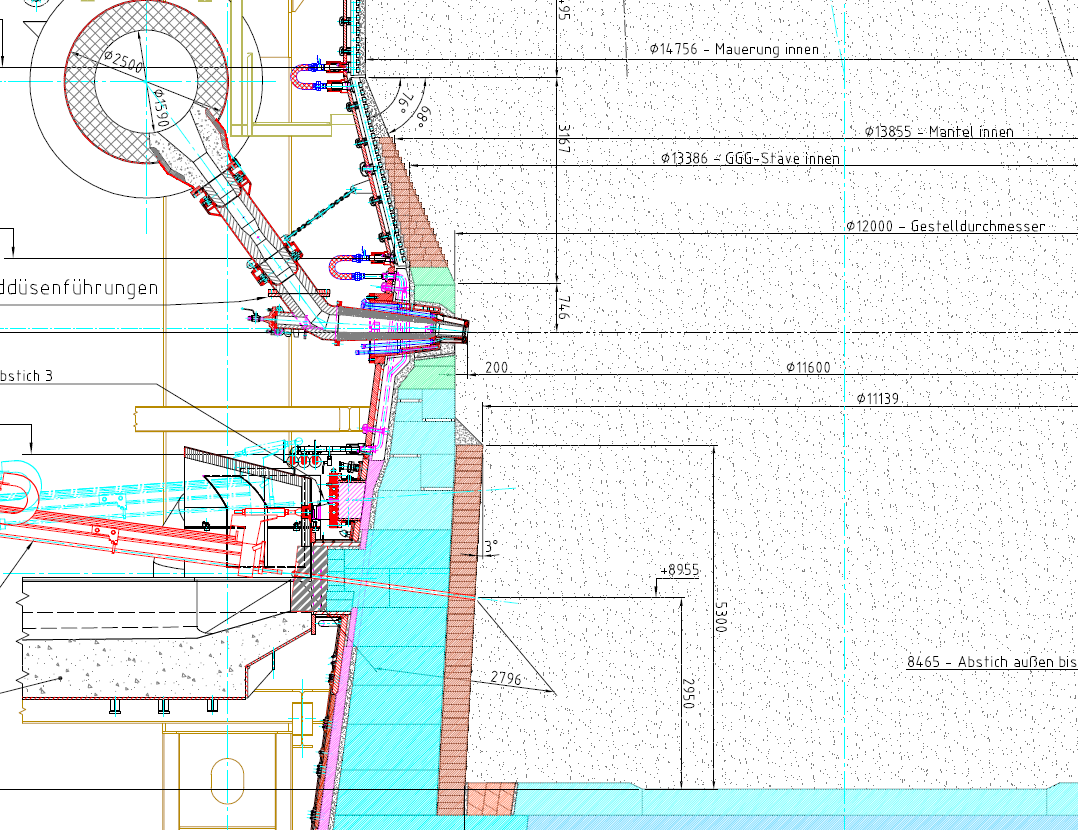
\includegraphics[width=.40\columnwidth]{images/068racewaylayout}
	  \label{fig:068racewaylayout}  }
  \\
  \caption{Schematics of the blast furnace investigation.}
  \label{fig:319raceway}
\end{figure}

\subsection{Structure}
\label{subsec:bfstructure}

The blast furnace is a massive vertical apparatus, built with consistent amounts
of refractory materials and a robust steel shell.
The areas in front of each tuyere, which can be seen in Fig.
\ref{fig:125blastfurnace}, is called $raceway$ and is the most active. 
We dedicated this chapter to the investigation of its behaviour.

\subsection{Simulation layout}
\label{subsec:simulationlayout}

Given its axial-symmetric geometry and according to \citet{RefWorks:208}, we
considered only a wedge and applied periodic boundary conditions.
Three tuyeres and a sufficiently high space over and under them were used to
grant uniform conditions.
As in \citet{RefWorks:208}, 15,000 cells were created for the mesh, shown in
Fig. \ref{fig:273layoutbf}. We performed a
limited number of simulations of this volume to investigate the effect of the
variation of the \acl{mus} (\acs{mus}).

\begin{figure}[!htb]
\centering
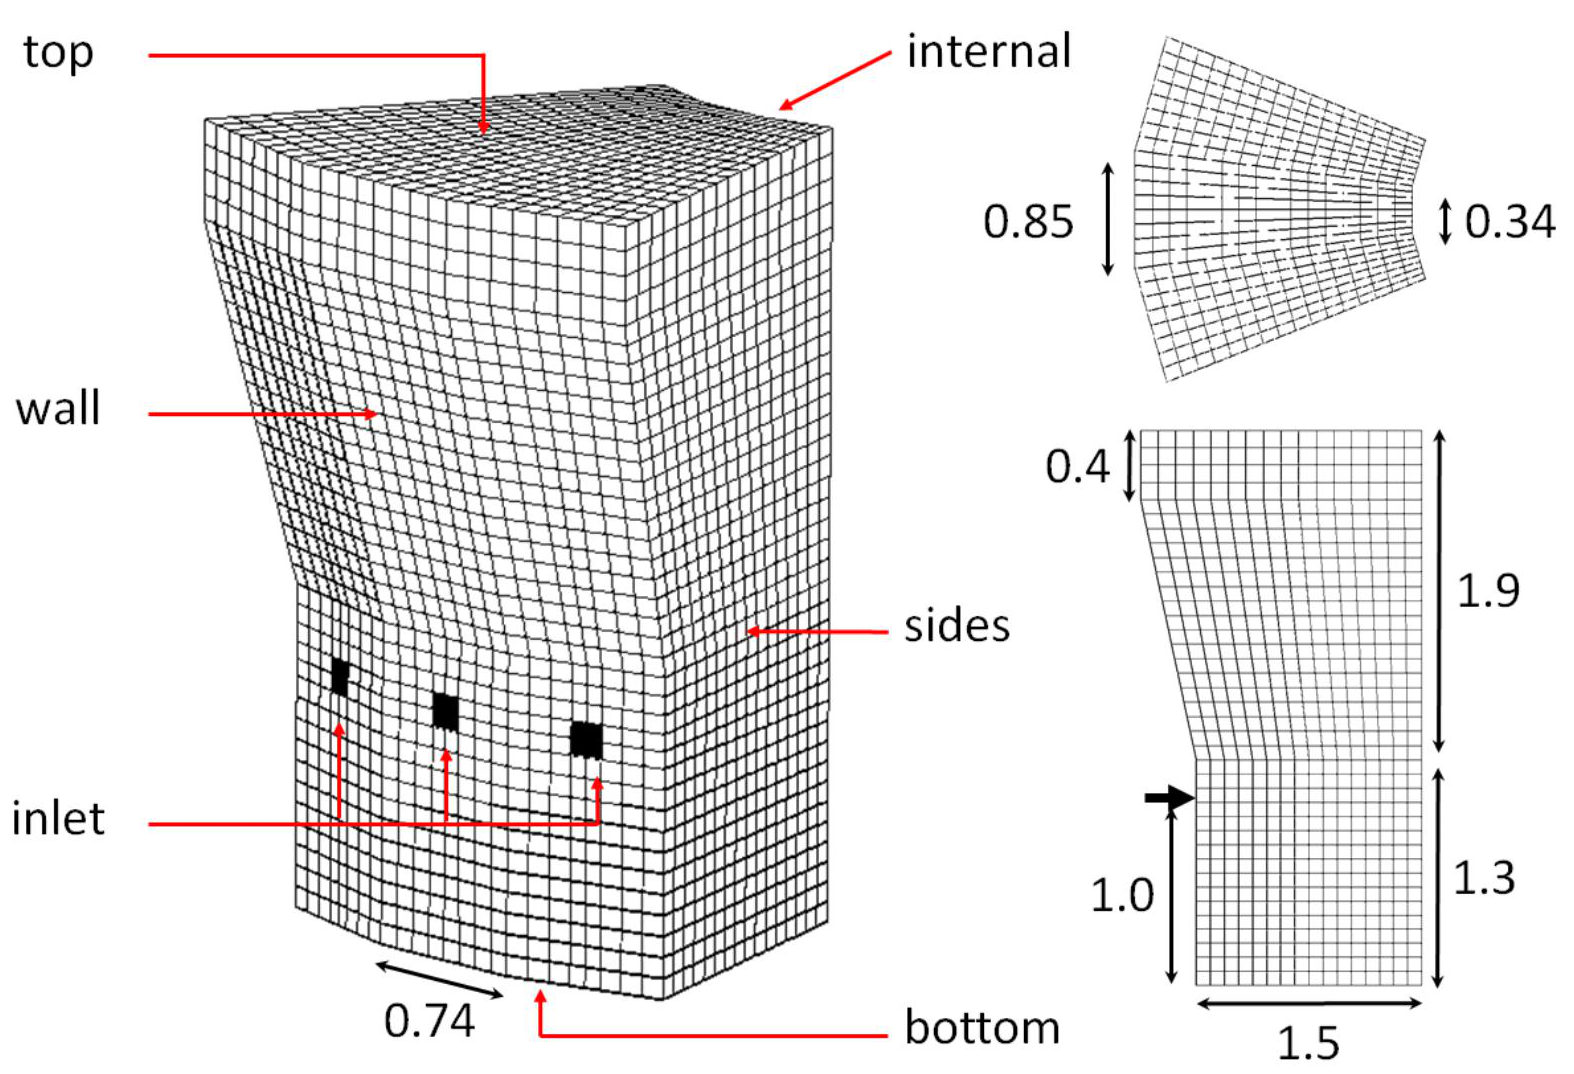
\includegraphics[width=.80\columnwidth]{images/273layoutbf}
\caption[Blast furnace simulation layout]{Blast furnace simulation layout \cite{RefWorks:208}.}
\label{fig:273layoutbf}
\end{figure}

\section{Results}
\label{sec:resultsbf}

\info{incomplete}

The change of sliding friction coefficients bear no effect on the
velocity of the gases. 
However, the particles velocity is clearly, and logically, higher for low
friction particles. 
They could be moved by the flow more easily compared to high
friction particles, see Fig. \ref{fig:300us_average_lf}.

\begin{figure}[htbp]
\centering 
  \subfloat[\acs{mus} = 0.1, spatial average.]
  {
	  
\includegraphics[width=.21\columnwidth]{images/288u_average_lf_stat}
	  \label{fig:288u_average_lf_stat}
  }
  \quad
    \subfloat[\acs{mus} = 0.1, velocity vectors.]
    {
	  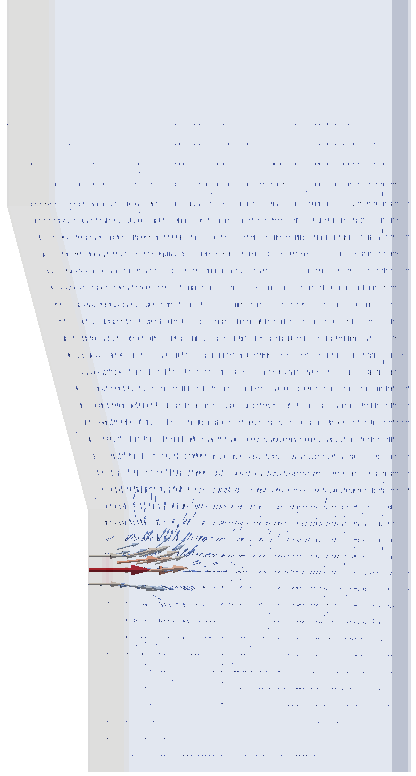
\includegraphics[width=.21\columnwidth]{images/287u_average_lf_arrow}
	  \label{fig:287u_average_lf_arrow}
  }
  \quad
    \subfloat[\acs{mus} = 0.1, stream lines.]
    {
	  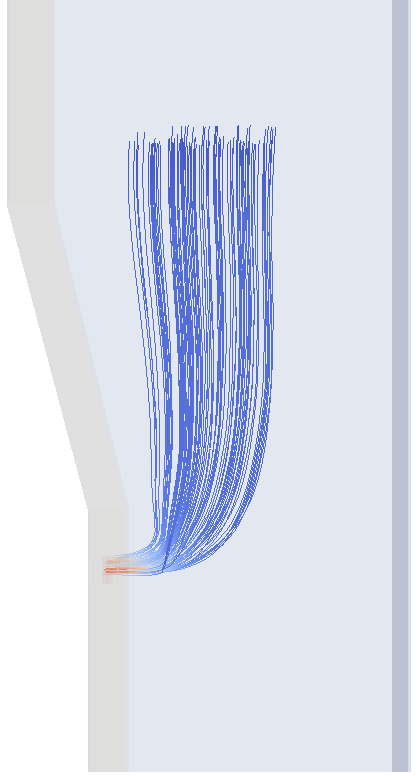
\includegraphics[width=.21\columnwidth]{images/289u_average_lf_stream}
	  \label{fig:289u_average_lf_stream}
  }
  \quad
  \subfloat[Legend.]
  {
	  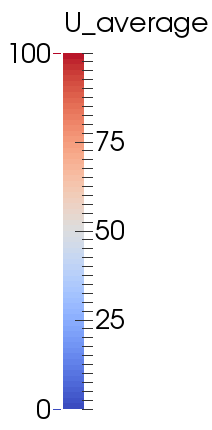
\includegraphics[width=.21\columnwidth]{images/274u_average_legend}
	  \label{fig:274u_average_legend}
  }
  \\
  \subfloat[\acs{mus} = 0.9, spatial average.]
  {
	  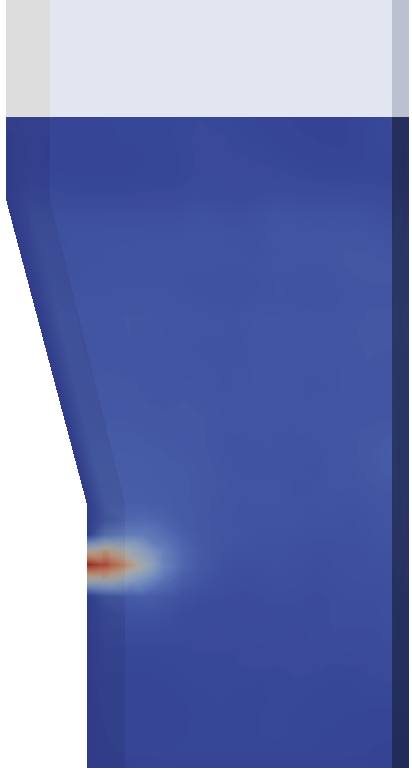
\includegraphics[width=.21\columnwidth]{images/276u_average_hf_stat}
	  \label{fig:276u_average_hf_stat}
  }
  \quad
    \subfloat[\acs{mus} = 0.9, velocity vectors.]
    {
	  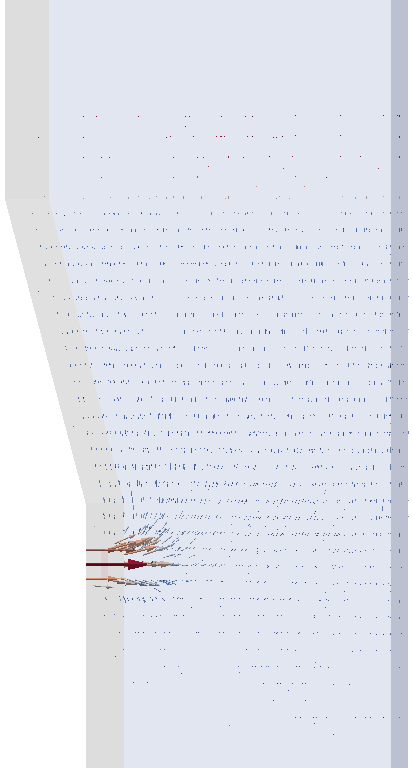
\includegraphics[width=.21\columnwidth]{images/275u_average_arrow}
	  \label{fig:275u_average_arrow}
  }
  \quad
    \subfloat[\acs{mus} = 0.9, stream lines.]
    {
	  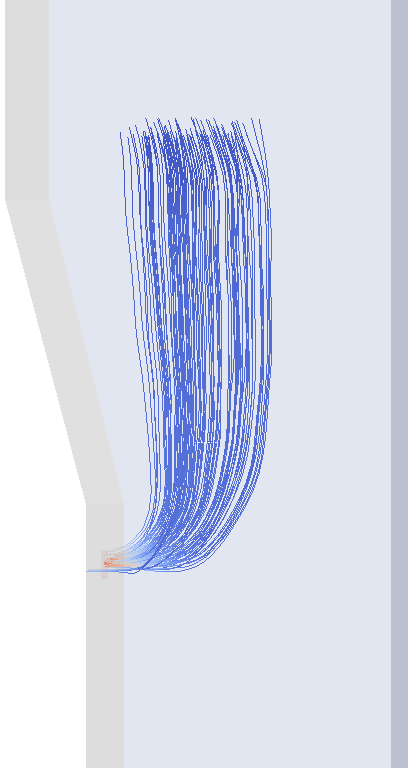
\includegraphics[width=.21\columnwidth]{images/277u_average_hf_stream}
	  \label{fig:277u_average_hf_stream}
  }
  \quad
  \subfloat[Legend.]
  {
	  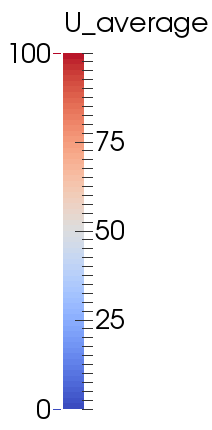
\includegraphics[width=.21\columnwidth]{images/274u_average_legend}
	  \label{fig:274u_average_legend}
  }
  \\  
  \caption[Vertical slice of fluid velocity]{Vertical slice of fluid velocity.}
  \label{fig:299u_average_lf}
\end{figure}
\begin{figure}[htbp]
\centering 
  \subfloat[\acs{mus} = 0.1, \acs{mur} = 0.4, $v_{inlet}$ = 100 m/s .]
  {
	  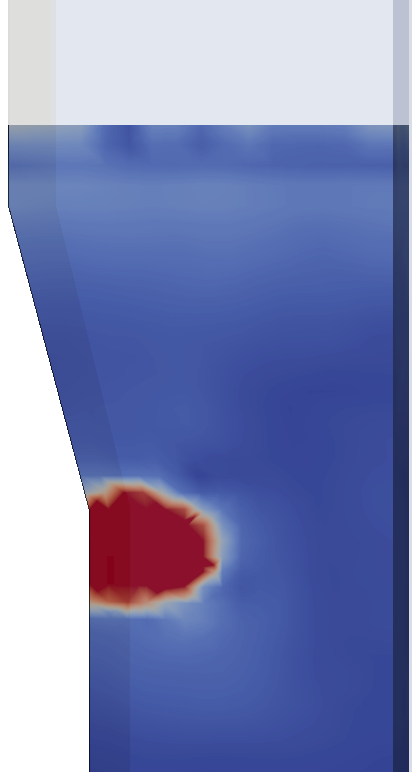
\includegraphics[width=.22\columnwidth]{images/291us_average_lf_stat}
	  \label{fig:291us_average_lf_stat}
  }
  \quad
    \subfloat[\acs{mus} = 0.5, \acs{mur} = 0.4, $v_{inlet}$ = 100 m/s .]
    {
	  
\includegraphics[width=.21\columnwidth]{images/290us_average_lf_arrow}
	  \label{fig:290us_average_lf_arrow}
  }
  \quad
    \subfloat[\acs{mus} = 0.9, \acs{mur} = 0.4, $v_{inlet}$ = 100 m/s .]
    {
	  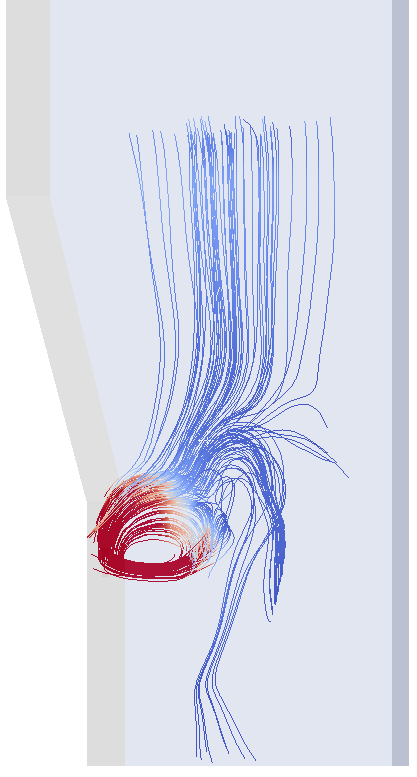
\includegraphics[width=.21\columnwidth]{images/292us_average_lf_stream}
	  \label{fig:292us_average_lf_stream}
  }
  \quad
  \subfloat[\acs{mus} = 0.1, \acs{mur} = 0.4, $v_{inlet}$ = 200 m/s .]
  {
	  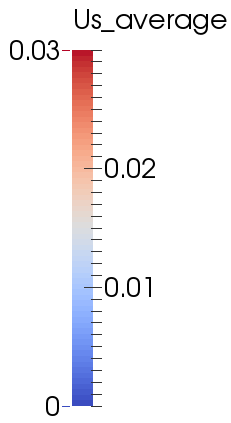
\includegraphics[width=.21\columnwidth]{images/278us_average_hf_legend}
	  \label{fig:278us_average_hf_legend}
  }
  \\
  \caption{300us_average_lf .}
  \label{fig:300us_average_lf}
\end{figure}

\begin{figure}[htbp]
\centering 
  \subfloat[\acs{mus} = 0.1, $u_{lim}$ = 4 m/s]
  {
	  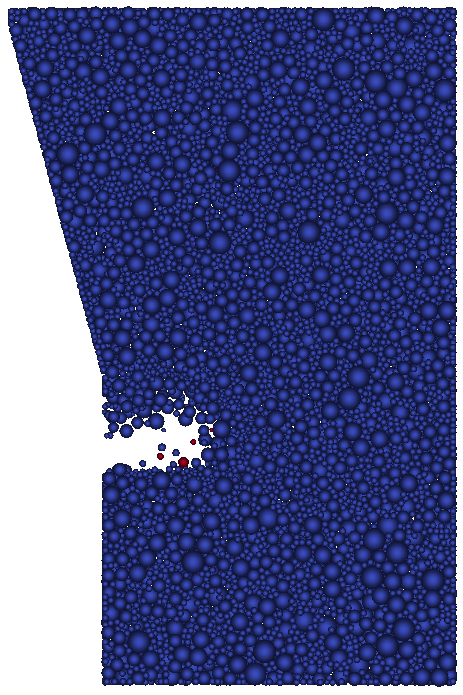
\includegraphics[width=.21\columnwidth]{images/296ver_slice_4mslf}
	  \label{fig:296ver_slice_4mslf}
  }
  \quad
    \subfloat[\acs{mus} = 0.1, $u_{lim}$ = 0.1 m/s]
    {
	  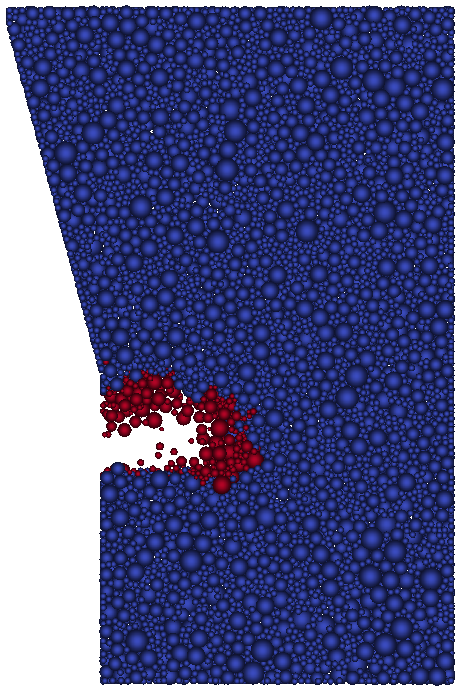
\includegraphics[width=.21\columnwidth]{images/295ver_slice_01mslf}
	  \label{fig:295ver_slice_01mslf}
  }
  \quad
    \subfloat[\acs{mus} = 0.1, $u_{lim}$ = 0.01 m/s]
    {
	  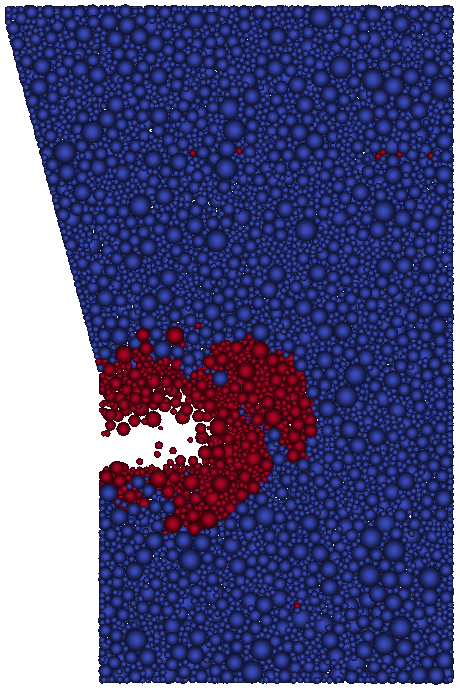
\includegraphics[width=.21\columnwidth]{images/294ver_slice_001mslf}
	  \label{fig:294ver_slice_001mslf}
  }
  \quad
  \subfloat[\acs{mus} = 0.1, $u_{lim}$ = 0.003 m/s]
  {
	  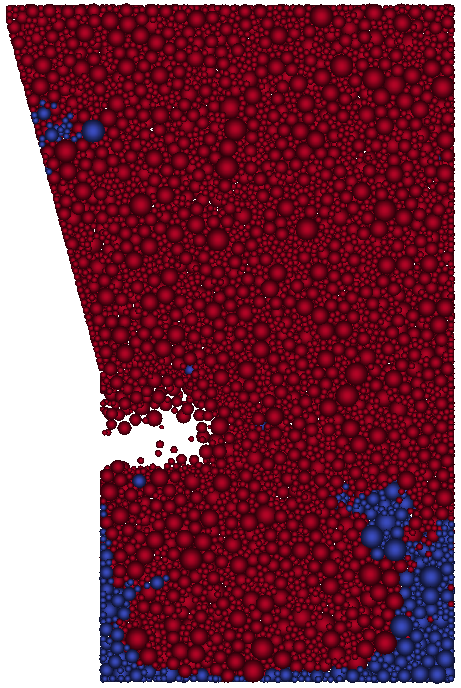
\includegraphics[width=.21\columnwidth]{images/293ver_slice_0003mslf}
	  \label{fig:293ver_slice_0003mslf}
  }
  \\
  \subfloat[\acs{mus} = 0.9, $u_{lim}$ = 4 m/s]
  {
	  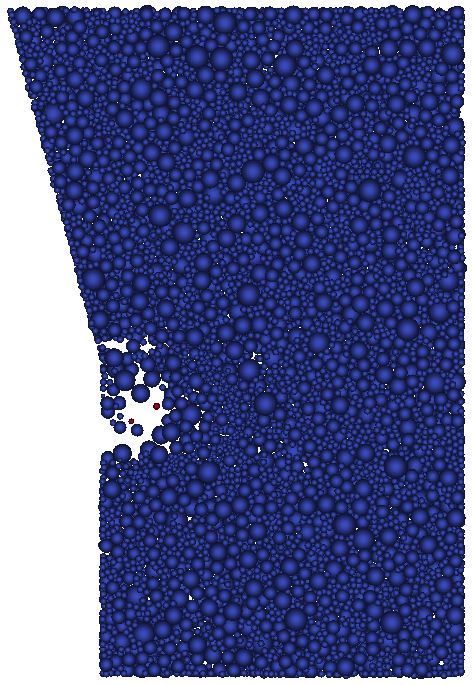
\includegraphics[width=.21\columnwidth]{images/266ver_slice_4mshf}
	  \label{fig:266ver_slice_4mshf}
  }
  \quad
    \subfloat[\acs{mus} = 0.9, $u_{lim}$ = 0.1 m/s]
    {
	  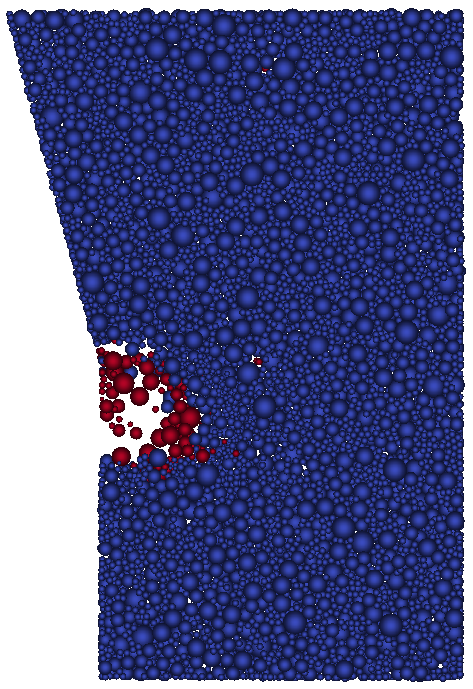
\includegraphics[width=.21\columnwidth]{images/267ver_slice_01mshf}
	  \label{fig:267ver_slice_01mshf}
  }
  \quad
    \subfloat[\acs{mus} = 0.9, $u_{lim}$ = 0.01 m/s]
    {
	  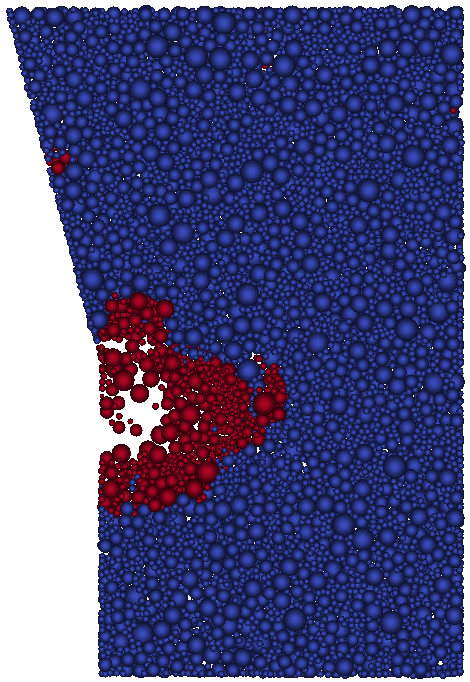
\includegraphics[width=.21\columnwidth]{images/268ver_slice_001mshf}
	  \label{fig:268ver_slice_001mshf}
  }
  \quad
  \subfloat[\acs{mus} = 0.9, $u_{lim}$ = 0.003 m/s]
  {
	  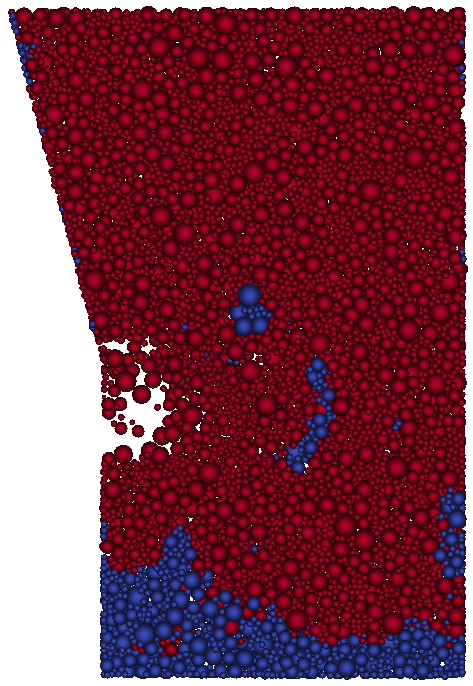
\includegraphics[width=.21\columnwidth]{images/269ver_slice_0003mshf}
	  \label{fig:269ver_slice_0003mshf}
  }
  \\  
  \caption[Vertical slice of particle velocity 2]{Vertical slice of particle
  velocity 2. Red particles are faster than the $u_{lim}$.}
  \label{fig:298verticalslicelf}
\end{figure}
\begin{figure}[htbp]
\centering 
  \subfloat[\acs{mus} = 0.1 .]
  {
	  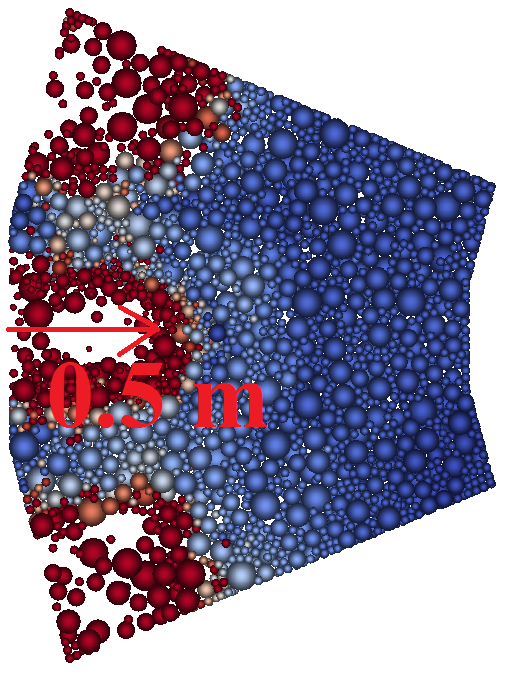
\includegraphics[width=.28\columnwidth]{images/285hor_slice_01mslf}
	  \label{fig:285hor_slice_01mslf}
  }
  \quad
    \subfloat[\acs{mus} = 0.9 .]
    {
	  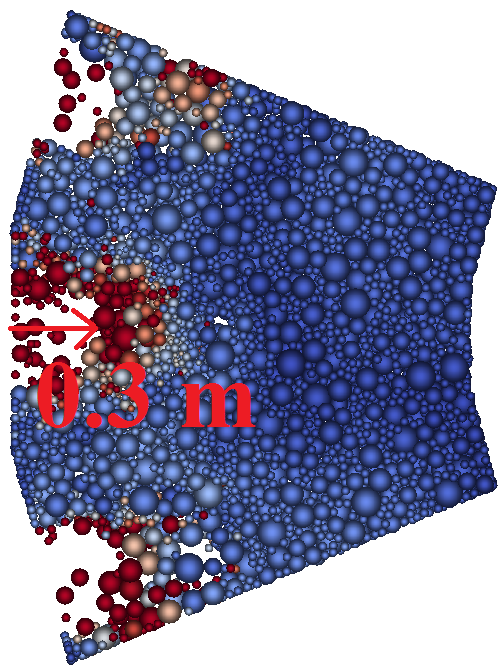
\includegraphics[width=.27\columnwidth]{images/271hor_slice_01mshf}
	  \label{fig:271hor_slice_01mshf}
  }
  \quad
    \subfloat[Legend and slice position.]
    {
	  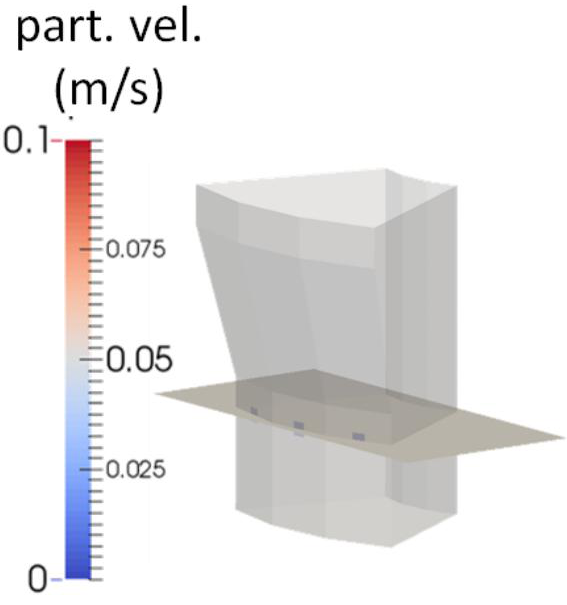
\includegraphics[width=.34\columnwidth]{images/272slice}
	  \label{fig:272slice}
  }
  \\
  \caption{Raceway penetration depth on the horizontal.}
  \label{fig:286hor_slice_01ms}
\end{figure}